\documentclass[aspectratio=169,dvipsnames,svgnames,10pt]{beamer}
\usepackage{minted}
\usepackage{alltt}
\usepackage[utf8]{inputenc}
\usepackage[T1]{fontenc}
\usepackage[english]{babel}
\usepackage{xspace}
\usepackage{cancel}
\usepackage{pifont}%% check mark
\usepackage{ stmaryrd }
\usepackage{wasysym}

\usepackage{lmodern}

\usepackage{natbib}
\bibliographystyle{abbrvnat}

\usetheme[sectionpage=none]{metropolis}
\setbeamercovered{transparent=20}
\usepackage[scaled=0.8]{DejaVuSansMono} % A decent mono font


\usepackage{tikz}
\usetikzlibrary{calc,fit,positioning,shapes,arrows,decorations.markings,backgrounds}
\newlength{\brickwidth}
\newlength{\brickheight}
\newlength{\brickdia}
\newlength{\brickdiaheight}
\newlength{\brickmultipliedx}
\newlength{\brickmultipliedy}
\newlength{\halfbrickwidth}
\setlength{\brickheight}{9.6mm}
\setlength{\brickwidth}{8mm}
\setlength{\brickdia}{2.8mm}
\setlength{\brickdiaheight}{1mm}
\setlength{\halfbrickwidth}{0.5\brickwidth}

\newcommand{\startpos}[3]
{($(0,#3\brickheight)+(7:#1\brickwidth)+(138:#2\halfbrickwidth)$)}
\newcommand{\startposplusheight}[3]
{($(0,#3\brickheight)+(7:#1\brickwidth)+(138:#2\halfbrickwidth)+(0mm,\brickheight)$)}
\newcommand{\pinposone}[5]
{($(0,#3\brickheight)+(7:#1\brickwidth)+(138:#2\halfbrickwidth)+(7:#4*\brickwidth)+(138:#5*\halfbrickwidth)+(-0.6\brickwidth,-\halfbrickwidth)+(-0.05\brickwidth,1.35\brickheight)$)}
\newcommand{\pinpostwo}[5]
{($(0,#3\brickheight)+(7:#1\brickwidth)+(138:#2\halfbrickwidth)+(7:#4*\brickwidth)+(138:#5*\halfbrickwidth)+(-0.6\brickwidth,-\halfbrickwidth)+(0.3\brickwidth,1.35\brickheight)$)}

\newcommand{\pin}[2]{%
  \filldraw[thick] #1 -- ++(0mm,-1.6\brickdiaheight) .. controls +(\brickdia,-0.1\brickheight) .. ++(2\brickdia,0mm) -- ++(0mm,1.6\brickdiaheight) -- cycle;
  \filldraw[thick] #2 ellipse[x radius=\brickdia, y radius=\brickdiaheight];
}

\tikzset{
  pics/brick/.style args={#1*#2 at #3,#4,#5}{code={
      \setlength{\brickmultipliedx}{#1\brickwidth}
      \setlength{\brickmultipliedy}{#2\brickwidth}
      \filldraw[thick]
      \startpos{#3}{#4}{#5} -- ++(7:\brickmultipliedx) -- ++(0mm,\brickheight) -- ++(138:0.5\brickmultipliedy) -- ++(187:\brickmultipliedx) -- ++(0mm,-\brickheight) -- cycle;
      \draw[thick] \startpos{#3}{#4}{#5} -- ++(0mm,\brickheight) -- ++(138:0.5\brickmultipliedy);
      \draw[thick] \startposplusheight{#3}{#4}{#5} -- ++(7:\brickmultipliedx);
      \foreach \i in {1,...,#1} {
        \foreach \j in {1,...,#2} {
          \pin{\pinposone{#3}{#4}{#5}{\i}{\j}}{\pinpostwo{#3}{#4}{#5}{\i}{\j}}
        }
      }
    }
  }
}

\definecolor{green}{rgb}{0, 0.5, 0.1}
\definecolor{magenta}{rgb}{1, 0, 0}
\newcommand{\error}[1]{\textcolor{red}{#1}}
\newcommand{\ok}[1]{\textcolor{green}{#1}}


\newcommand\Y{{\color{Green}{\ding{52}}}\xspace}
\newcommand\N{{\color{Red}{\ding{56}}}\xspace}
\newcommand\M{{\color{Orange}{\bf\textasciitilde}}\xspace}

\title{A Tour of ML-style module systems}
\author{Gabriel Radanne}
\date{}

\begin{document}

\maketitle

\begin{frame}
  \frametitle{Programming like Legos}

  When programming software, we want \emph{modularity} and \emph{abstraction}
  \begin{itemize}
  \item Modularity/Separation of concern: Reusable independent bundles of code
  \item Abstraction/Encapsulation: Hide irrelevant implementation details
  \end{itemize}

  Many ``programming units'' in various languages: Packages, Modules, Crates, Components \dots

  \large The goal: allow to assemble programs like
  Legos
  \resizebox{!}{1em}{\tikz{\pic[draw=black,fill=Chartreuse] {brick={2*2 at 0,0,0}};}}

  \begin{center}
    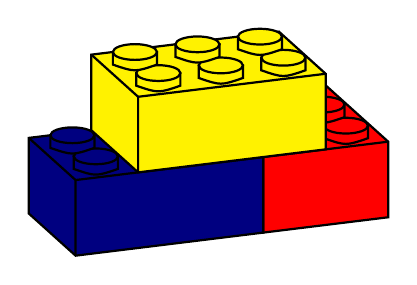
\begin{tikzpicture}
      \pic[draw=black,fill=red] {brick={2*4 at 2,0,0}};
      \pic[draw=black,fill=NavyBlue] {brick={3*2 at -1,0,0}};
      \pic[draw=black,fill=yellow] {brick={3*2 at 0,0,1}};
    \end{tikzpicture}
  \end{center}

\end{frame}

\begin{frame}
  \frametitle{ML Modules}

  In many programming languages, assemblage is \emph{outside the main language}.\\
  Examples: Crates in Rust, Compilation Units in Haskell, \dots

  ML Modules are \emph{constructs inside the language} for programming in the large!

  \LARGE\[
    \tt module\ F(\resizebox{!}{1em}{\tikz{\pic[draw=black,fill=red] {brick={2*2 at 0,0,0}};}})
    = 
    \resizebox{!}{2em}{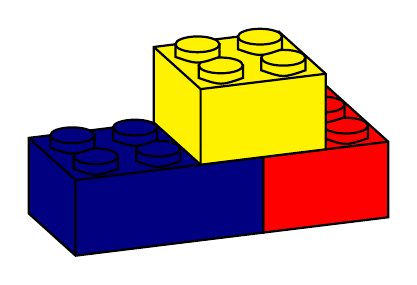
\begin{tikzpicture}
        \pic[draw=black,fill=red] {brick={2*4 at 2,0,0}};
        \pic[draw=black,fill=NavyBlue] {brick={3*2 at -1,0,0}};
        \pic[draw=black,fill=yellow] {brick={2*2 at 1,0,1}};
      \end{tikzpicture}}
  \]
\end{frame}

\begin{frame}
  \centering\Huge Demo time in OCaml
\end{frame}

\begin{frame}
  \frametitle{OCaml Modules: A recap}

  Modules form a typed sub-language of OCaml for programming in the large

  Features:
  \begin{itemize}
  \item Small $\lambda$-calculus
  \item Qualified accesses
  \item Large-scale name-aware operations (open, include, \dots)
  \item Structural Subtyping
  \item Identity is important: Aliases, Dependent arrows, \dots
  \end{itemize}
  
\end{frame}

\begin{frame}[fragile]{A core OCaml module system}
  Today's glimpse at the theory: Core OCaml modules \citep{Leroy94,Leroy95,Leroy96}
  \begin{itemize}
  \item Applicative functor -- \mintinline{ocaml}{Map.Make(String)}
  \item Module ascription -- \mintinline{ocaml}{(M : S)}
  \item Manifest -- \mintinline{ocaml}{type foo = Foo.t = MyFoo}
  \item Qualified access -- \mintinline{ocaml}{A.v}, \mintinline{ocaml}{F(X).t}
  \end{itemize}
\end{frame}

\begin{frame}{Core OCaml: Warming up}

  The important judgements:
  \begin{center}
  \includegraphics[width=0.6\linewidth]{judgements.png}
\end{center}

  A simple warm-up rule:
  \begin{center}
  \includegraphics[width=0.6\linewidth]{betared.png}
\end{center}
  
\end{frame}

\begin{frame}[fragile]{Core OCaml: Qualified accesses}

  Qualified accesses are not as trivial as expected:
  \begin{center}
  \includegraphics[width=0.5\linewidth]{qualifiedaccess.png}
\end{center}

  Example:

\begin{minted}{ocaml}
module X = sig 
  type t
  module A : sig val a : t end
end
\end{minted}

  We have $\Gamma \vdash$~\mintinline{ocaml}{X.A : sig val a : X.t end}

  $\Rightarrow$ Same pattern for all qualified accesses (types, values, modules, \dots)
  
\end{frame}

\begin{frame}{Core OCaml: Subtyping}

  Subtyping is \emph{Structural} on signatures:
  \begin{center}
  \includegraphics[width=0.9\linewidth]{subtypingstructure.png}
\end{center}

  This allows an arbitrary reordering of a subset of the fields.\\
  We then check fields by fields:

  \includegraphics[width=\linewidth]{subtypingfields.png}
  
\end{frame}

\begin{frame}[fragile]
  \frametitle{Core OCaml: Subtyping -- Example}
  
  A reasonably complex example of subtyping:
  \begin{columns}
    \begin{column}{0.5\textwidth}
      
\begin{minted}{ocaml}
module FooBar : sig
  type foobar = Foo | Bar
  type fbl = foobar list
  val singleton : foobar -> fbl
  val rev : fbl -> fbl
  val merge : fbl -> fbl -> fbl
end
\end{minted}
    \end{column}
    \begin{column}{0.5\textwidth}
      

\begin{minted}{ocaml}
module Fbl = (FooBar : sig
  type fbl
  val rev : fbl -> fbl
  val merge : fbl -> fbl -> fbl
  val singleton : FooBar.foobar -> fbl
end)
\end{minted}
    \end{column}
  \end{columns}
  \vfill

  \begin{columns}
    \begin{column}{0.5\textwidth}
      Subtyping allows us to:
      \begin{itemize}
      \item Reorder and hide some fields
      \item Replace types by equivalent ones
      \item Abstract some type definitions
      \end{itemize}
    \end{column}
    \begin{column}{0.5\textwidth}
      \includegraphics<2>[width=\linewidth]{subtyping16.png}
      \includegraphics<3>[width=\linewidth]{subtyping18.png}
    \end{column}
  \end{columns}
\end{frame}

\begin{frame}[fragile]
  \frametitle{Core OCaml: Strengthening}

  Applicative behavior is achieved through a new \emph{strengthening} operation $M/p$
  
  This operation ``strengthen'' a module type by adding additional type equalities.
  \vfill
  
  \begin{columns}
    \begin{column}{0.5\textwidth}
      Example:
\begin{minted}{ocaml}
module F (A : S) : sig type t val v : t end
\end{minted}

      Then we have:
      \mintinline{ocaml}{((A : S) -> sig type t val v : t end)}$/F =$\\
      \mintinline{ocaml}{(A : S) -> sig type t = F(A).t val v : t end}
      
    \end{column}
    \begin{column}{0.5\textwidth}
      \includegraphics<2>[width=\linewidth]{strengthening.png}
    \end{column}
  \end{columns}

\end{frame}

\begin{frame}
  \frametitle{Core OCaml: Inference}
  \begin{columns}
    \begin{column}{0.4\textwidth}
      In the original rules, subtyping and strengthening are free-floating:
      \begin{center}
        \includegraphics[width=.8\linewidth]{subtyp.png}

        \includegraphics[width=.35\linewidth]{strength.png}
      \end{center}
    \end{column}
    \begin{column}<2->{0.6\textwidth}
      We can coalesce them into Application/Declaration:
      \begin{center}
        \includegraphics<2->[width=.9\linewidth]{inference.png}
      \end{center}
    \end{column}
  \end{columns}
  \vspace{3em}
  \visible<3>{$\Rightarrow$ This immediately yield an inference algorithm}
\end{frame}

\begin{frame}
  \frametitle{OCaml: The rest}

  There are many things not covered in this core language:
  \begin{itemize}
  \item Generative functor
  \item \texttt{with} constraints
  \item \texttt{module type of}
  \item First class modules
  \item Module aliases
  \item Recursive modules
  \end{itemize}

  Some (but not all) are covered by other formalizations\\
  $\Rightarrow$ Still lot's of work!
\end{frame}

\begin{frame}
  \frametitle{Modules: Metatheory}

  What kind of meta-theoretical result can we expect from module systems ?
  \begin{itemize}
  \item Soundness\\
    Might seem obvious, but very complicated for modules due to abstract types
  \item Representation Independence (Similar to Reynold's abstraction)\\
    \begin{quote}
      Let $m_1$ and $m_2$ be two closed module expressions of type $M$.
      Assume $m_1$ and $m_2$ are ``equivalent'' (to be defined).
      For all program contexts $C[ ]$ such that $x : M \vdash C[x]$, we have
      $\llbracket C[m_1] \rrbracket = \llbracket C[m_2] \rrbracket$.
    \end{quote}
  \item Incremental typechecking\\
    \begin{quote}
      Given a list of module declarations that form a typed program, there exists an order such that each module can be typechecked with only knowledge of the type of the previous modules.
    \end{quote}
  \end{itemize}
  
\end{frame}

\begin{frame}{Other ML module systems}

  Debates and tradeoffs:
  \begin{itemize}
  \item ``Applicative'' vs. ``Generative'' functors
  \item How separated are the core and module languages?
  \item What about recursive modules?
  \item Style of formalisation: syntactic, semantic, \dots
  \end{itemize}

  \visible<2>{$\Rightarrow$ Let's do a quick tour of the various approaches}
  
\end{frame}


\begin{frame}{OCaml}

  OCaml (circa. 1996), is a mainstream language/compiler:
  \begin{itemize}
  \item[\M] Partial formalization \citep{Leroy94,Leroy95,Leroy96}\\
    Uses \emph{syntactic} rules
  \item[\N] Nothing mechanized
  \item[\Y] Both applicative and generative functors
  \item[\Y] Separate compilation
  \item[\Y] Numerous extensions:\\
    First class modules, module aliases, private, \texttt{with} constraints, \dots\\
    Towards less stratified and more dependent languages.\\
    \N Not formalized. Interactions unclear (... or unsound)
  \end{itemize}
  
\end{frame}


\begin{frame}[fragile]{Real OCaml: Aliases and functors}

  An example of delicate interactions: It is not sound to create an alias of a functor parameter.
\begin{minted}{ocaml}
module F (X : S) = struct
  module A = X (* this is not an alias *)
end
\end{minted}
  {\bf Why}: if the alias is kept, \only<2->{{\color{Grey} we could discover that
  \texttt{F(MyModule).A = MyModule}, and thus discover fields that are not in
  \texttt{S}. Since module coercions are implemented by copies, }}that might lead to segfaults\only<1>{?!?}.

    \begin{onlyenv}<3>
  {\bf Currently}: The type is expanded and module equality is lost:
\begin{minted}{ocaml}
module F (X : S) : sig
  module A : S with type t = X.t
end
\end{minted}
\end{onlyenv}
  
\end{frame}

\begin{frame}{Standard ML}

  Standard ML (1983) is a \emph{standard} implemented by several compilers: MLTon, SMLNJ, \dots
  \begin{itemize}
  \item[\Y] Fully formalized \citep{MacQueen84}\\
    Uses \emph{semantic} objects (strong sums, notably)
  \item[\Y] Fully mechanized! \citep{Crary17,Crary19}
  \item[\N] Only \emph{generative} functors. High order limited
  \item[\M] Partial Separate compilation~\citep{DBLP:conf/ml/SwaseyVCH06}
  \item[\Y] Many new features formalized:\\
    First class modules~\citep{Russo00}, module aliases~\citep{Crary17}, \dots\\
    \N But none of them implemented
  \end{itemize}
  
\end{frame}

\begin{frame}
  \frametitle{Collection of Modules ideas}

  Language extensions:
  \begin{itemize}
  \item The (never ending?) quest towards recursive modules~\citep{dreyerthesis}\\
    $\Rightarrow$ Still very very complicated
  \item Modules for Haskell~\citep{backpack}\\
    An \emph{external} language. Allow to arrange linking of compilation units
  \item Mixin and Modules~\citep{DBLP:journals/toplas/RossbergD13}\\
    Offer a promising alternative solution to recursive modules!
  \end{itemize}
  \vfill
  \pause
  Doing other things with modules:
  \begin{itemize}
  \item Modular Macros~\citep{modularmacrosth}
  \item Distributed programming \citep{acute}
  \item Client-server programming: My thesis \smiley{} \citep{radannethesis}
  \item Operating systems~\citep{DBLP:conf/asplos/MadhavapeddyMRSSGSHC13,DBLP:journals/corr/abs-1905-02529}
  \end{itemize}
 
\end{frame}

\begin{frame}
  \frametitle{F-ing modules and 1ML}

  F-ing module~\citep{FingModules}: Translate modules into system $F_w$!
  \begin{itemize}
  \item[\Y] Gives a \emph{much} simpler/nicer proof of soundness
  \item[\Y] Supports applicative/generative, inference, aliases, \dots
  \item[\N] Formalization only defined by \emph{translation}\\
    $\Rightarrow$ How to surface back the result?
  \end{itemize}

  Examples of translation:
  \begin{itemize}
  \item Abstract types $\to$ Existentials
  \item Module subtyping $\to$ Record subtyping
  \item Functors $\to$ High order polymorphic functions
  \item Aliases $\to$ Singletons
  \end{itemize}

  1ML~\citep{DBLP:journals/jfp/Rossberg18} uses this translation
  to build a language with \emph{unified core and module languages}.
\end{frame}

\begin{frame}
  \frametitle{Conclusion}

  In this presentation, We explored ML modules:
  \begin{itemize}
  \item ML modules in practice in OCaml
  \item A core OCaml calculus
  \item Glimpses of some other ML calculus
  \end{itemize}
  \pause

  What I want you to remember:
  \begin{itemize}
  \item ML modules are \emph{fantastic} tools for large-scale programming.\\
    Scales extremely well to the size of the ecosystem
  \item Module formalization does not have to be daunting.\\
    A syntactic approach is accessible, and F-ing provides new very powerful tools
  \item Still, lot's of work remains!\\
    $\Rightarrow$ I'm current working on a much more complete formalization of OCaml modules
  \end{itemize}

  Hopefully, you should be well equipped to dive deeper into the literature!
  
\end{frame}

\bibliography{../biblio.bib}


\appendix

\begin{frame}[fragile]{Status of the module system -- The less good}
  What about ``recent'' features ?
  \begin{itemize}
  \item Generative functor:
    Well understood \Y
  \item \texttt{with} constraints: 
    No real formalization \N
  \item \texttt{module type of}:
    No formalization, Uncertain semantics \N
  \item First class modules:
    Formalized as ``package types'' \Y ...
    but only in SML \N
  \item Module aliases:
    Well studied in theory as singletons \Y ...
    but in very different settings \N
  \item Private fields:
    Only partial formalization
  \item<2>
    Interactions are not always clear
  \end{itemize}
\end{frame}



\begin{frame}{Another look at the module system}

  \textbf{Goal}: Let's have a new look at module formalization:
  \begin{itemize}
  \item Reconcile the problematic pieces
  \item Think about inference
  \item Fix/improve the known problems
  \item Provide a sure footing for further experimentation (modular implicits, \dots)
  \end{itemize}

  \pause
  \textbf{Non-goal}: Design a new language. 1ML is cool, but we can't use it.

  \pause
  Let's look at some of the big problems!
\end{frame}



\begin{frame}[fragile,fragile]{The Ugly -- Part 1\hfill Aliases and functors}
  
  {\bf Problem}: It is not sound to create an alias of a functor parameter:
\begin{minted}{ocaml}
module F (X : S) = struct
  module A = X (* this is not an alias *)
end
\end{minted}
  {\bf Why}: if the alias is kept, \only<2->{{\color{Grey} we could discover that
  \texttt{F(MyModule).A = MyModule}, and thus discover fields that are not in
  \texttt{S}. Since module coercions are implemented by copies, }}that might lead to segfaults\only<1>{?!?}.

    \begin{onlyenv}<3>
  {\bf Currently}: The type is expanded and module equality is lost:
\begin{minted}{ocaml}
module F (X : S) : sig
  module A : S with type t = X.t
end
\end{minted}
\end{onlyenv}
  
\end{frame}

\begin{frame}[fragile]
  \frametitle{Transparent ascriptions}

  {\bf Solution}: Transparent ascriptions!

  Transparent ascriptions hide the values but keep the types.
\begin{minted}{ocaml}
module F (X : S) : sig
  module A = (X <: S) (* X viewed through S *)
end
\end{minted}

  \pause
  \begin{itemize}
  \item A ``filter'' on the dynamic part of the module
  \item Also in path : \texttt{F(Y <:\ S).A}
  \item Generally useful for ``soft constraints'':
\begin{minted}{ocaml}
module MyKey <: Map.OrderedType = ...
\end{minted}
  \item Essential for modular implicits
  \end{itemize}
  
\end{frame}

\begin{frame}[fragile]
  \frametitle{The Ugly -- Part 2\hfill Eager operations}

  \textbf{Problem}: Many operations on modules are expanded eagerly: \texttt{with}, \texttt{include}, \texttt{module type of}, strengthening, \dots
  \begin{itemize}
  \item Lead to big signatures (Eliom has $>5$Mo {\tt .cmi}, Janestreet has build perf issues, \dots)
  \item Loose the original information, problematic for errors and tools (documentation, notably)
  \end{itemize}

  \pause
  \textbf{Currently}, when you type:
\begin{minted}{ocaml}
module type S = sig 
  val x : string
  module A : T
end
module M : S with type A.t = int
\end{minted}

  the typechecker understands:
\begin{minted}{ocaml}
module M : sig  val x : string  module A : sig type t = int ... end  end
\end{minted}
\end{frame}

\begin{frame}[fragile]{Incrementality}
  
  \textbf{Solution}: Make an \emph{incremental} calculus for modules.
  \begin{itemize}
  \item In a nutshell ``memoization for module type operations''.
  \item Similar to explicit substitutions, but on modules
  \item Need to be extra careful around environments!
  \end{itemize}

  When we typecheck ``\texttt{let y = M.x}'', we push only one step:
\begin{minted}{ocaml}
module M : sig
  val x : string
  module A : T with type t = int
end
\end{minted}
\end{frame}

\begin{frame}{Current status}

  {\bf In progress}:
  \begin{itemize}
  \item Core of the specification is done
  \item Prototype ``clean room'' implementation in progress
  \end{itemize}

  {\bf To be done}:
  \begin{itemize}
  \item Progressively add more and more features
  \item Prove good properties
  \end{itemize}
\end{frame}

\begin{frame}[fragile,fragile,fragile]
  \frametitle{The Ugly -- Part 3\hfill The avoidance problem}

  \textbf{Problem} Let's write the this C\&C (cool and contrived) functor:
\begin{minted}{ocaml}
module F (X : S) = struct
  type a = X.t list
  type b = X.t * int
end
\end{minted}

  What's the type of:
\begin{minted}{ocaml}
module A = F(struct type t = A | B end)
\end{minted}
  \pause
  The typechecker gives us:
\begin{minted}{ocaml}
module A : sig type a type b end
\end{minted}
  This is not very useful. 
\end{frame}

\begin{frame}[fragile,fragile]{Local bindings and inference}

  We want to have a \emph{principal module type} for this.
  \begin{itemize}
  \item This type is used for inference
  \item It does not have to appear in user signatures
  \end{itemize}
  \pause
  
  {\bf Solution}: Local module types:
\begin{minted}{ocaml}
module A : let X : ... in sig
  type a = X.t list
  type b = X.t * int
end
\end{minted}

  We can then simplify this further down (incrementally, as before).
\end{frame}

\end{document}

%%% Local Variables:
%%% mode: latex
%%% TeX-command-extra-options: "-shell-escape"
%%% TeX-master: t
%%% End:
